
%%% Local Variables: 
%%% mode: latex
%%% TeX-master: "main"
%%% End: 
\section{Exploratory Tools}
% This section should first describe why an exploratory tool was needed. Second, why was an interactive tool needed? Be brief.

 Close inspection and description of the background signal was required to identify and address the previously mentioned misassemblies. Such illustration is typically accomplished with a genome browser. Genome browsers allow the exploration of sequencing datasets in high detail, producing publication-ready images of coverage, mutations, and more. Several features were required from a genome browser to characterize the misassemblies and enable assembly curation. 

Specifically, an ideal genome browser would display coverage and annotation data from both strands separately. Visualization of multiple coverage vectors (e.g. different conditions) in a single track is preferable to multi-track browser designs. Unfortunately, ``reducer'' functions (max, sum, average) are not simple to compute for multiple large alignment files and existing genome browsers. In fact, many conventional browsers are sluggish to even load such large datasets. These genome browsers (IGV, UCSC genome browser, Gbrowse) did not meet the requirements for this project. Instead, a customized genome browser was constructed with flexibility, speed, and simplicity in mind to facilitate assembly visualization and curation with the sequencing data and genome annotations.

\begin{wrapfigure}{R}{0.4\textwidth}
\small
\vspace{-20pt}
\begin{center}
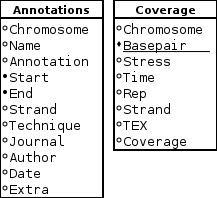
\includegraphics[width=0.38\textwidth]{images/Assembly/Browser/Genome_browser_schema.png}
\end{center}
\vspace{-20pt}
\caption{Database Tables}\label{fig:5.5}
A simple database was designed, indexing the annotations and coverage entities on their genomic coordinates.
\end{wrapfigure}

\subsubsection{Genome Browser}
In this genome browser, only the coverage vector was required for visualization and not the inspection of individual reads. A total of 169 gigabytes of aligned reads were summarized by 6.8 gigabytes of coverage vectors. This data was too large to transmit to users or perform reducing functions upon. The appropriate format for visualization and distribution of these data was a web application with a database. The objective for this genome browser was simple: allow users to upload and view feature annotations (e.g. sRNAs, proteins) alongside condition-specific coverage vectors from this sequencing dataset. The details of its construction are described in the Methods chapter (reference methods genome browser).

The finished product is a modern genome browser with an intuitive user interface(\ref{app:browser_ui}). A simple database was required to host coverage and annotation records, to be retrieved and converted into scalable vector graphics (SVG). This tool is both fast and flexible with optimized queries and interactive zooming, filtering, and tooltip details. Strand specific coverage and annotations are displayed in a publication ready form. The genome browser is a tool to integrate annotation types including the transcriptome assembly, reference CDSes, and more, contextualizing these genomic features with expression data. After construction, this genome browser was loaded with genome annotations to facilitate error correction.

\subsubsection{Promoter Prediction Tool}
To aid the curation process, it was desirable to integrate additional annotations such as promoter and terminator predictions. Unfortunately, quality promoter annotations do not exist for \textit{C. acetobutylicum}. The extension and fusion misassemblies resulted from residual background signal near transcript termini; the precision of transcription start site determinations could have been improved with genome-wide prediction of promoter motifs and transcription factor binding sites.


Genome annotations, such as promoter predictions, can help resolve various misassemblies such as extensions and fusions. A promoter prediction tool was developed to utilize consensus sequences from \textit{B. subtilis} to predict promoter motifs in this \textit{C. acetobutylicum}. The promoter prediction tool, described in \ref{methods:promoter_prediction}, converts consensus sequences into models suitable for input into the MAST algorithm (reference MEME suite/MAST algo). Consensus sequences from DBTBS (reference DBTBS) were used to generate models of promoter elements and transcription factor binding sites. Then, these were used to scan the \textit{C. acetobutylicum} genome. Predictions with p \textless 0.01 were then converted to GTF format and uploaded into the browser. This browser, loaded with annotations, was then used to visualize the errors and misassemblies in the uncurated assembly.

These exploratory tools were created to improve the precision of the transcript boundary estimates by contextualizing the coverage patterns with annotations (e.g. Rho-independent terminators) that explain drops in depth. These genomic signals suggest biological mechanisms for the observations, increasing the amount of signal present at transcript boundaries. This customized genome browser was used for integrative analyses of these genomic signals and sequencing data. 




